% Generated from: Zhihu/专栏：概率与统计/稳定分布：方差无穷时的中心极限定理_金鱼马_2026-04-11.md
\section{极限分布}
回顾一下定义~\ref{def:ch1:limit-distribution} 对``极限分布" 的定义，简单起见我们只考虑一维的情况，
\begin{definition*}[极限分布]
若一列（一维）随机变量 $\{X_n\}$ 满足：存在常数数列 $a_n$、$b_n>0$ 和某个（非退化）分布 $F$，使得 $b_n^{-1}(X_n-a_n)\overset{\rm d}\to F$，
就称 $\{X_n\}$ 的\emph{极限分布} 或 \emph{渐近分布 }是 $F$ 。
\end{definition*}

% 这个概念可以推广到高维，只需把 $X_n$ 换成 $k$ 维随机向量、 $a_n$ 换成 $\mathbb R^k$ 中的向量、 $b_n$ 换成 $k\times k$ 正定矩阵即可，简单起见我们都只考虑一维的情况。

看了这个定义后，我们自然会问：怎么选择 $a_n\in\mathbb R$ 和 $b_n>0$ ，使得 $\frac{S_n-a_n}{b_n}\overset{\rm d}\to F$ ？如果使用不同的中心化和归一化参数 $a_n,b_n$ ，是否会收敛到不同的极限分布？答案是否定的，下面的定理~\ref{thm:ext-stable:convergence-types}说明：极限分布如果存在，它们总是``同一类''的。

首先，容易见到，若\[ b_n^{-1}(X_{n}-a_n)\overset{\rm d}\to Z\sim F(x) \]

那么对任意常数 $c>0$ 和 $d\in\mathbb R$，我们总可以通过取 $b_n'=cb_n$ 和 $a_n'=a_n+db_n$，使得
\[
b_n'^{-1}(X_{n}-a_n')=\frac1c(b_n^{-1}(X_n-a_n)-d) \overset{\text{d}}\to \frac1c(Z-d)\sim F(cx+d).
\]

故此，作为极限分布，我们总可以将 $F(x)$ 和 $F(cx+d)$ 视作是等效的。

\begin{definition*}[同型分布]
若两个分布函数 $F_1$ 和 $F_2$ 满足：存在常数 $c>0$ 和 $d$ 使得 $F_1(x)=F_2(cx+d)$ 对任意 $x$ 成立，那么称这两个分布 $F_1$ 和 $F_2$ 是\textbf{\emph{同一类的}} (of the same type)。
\end{definition*}

直观上，只要两个分布可以通过横坐标的拉伸/压缩（乘以常数 $c$）和左右平移（加上常数 $d$）完全重合，我们就认为它们拥有相同的``核心形状''。显见，这个``同一类''关系是一个等价关系，它将全体一维分布函数划分为一些互不相交的等价类。

\begin{theorem}[收敛型定理]
\label{thm:ext-stable:convergence-types}

设 $F,G$ 是两个 (非退化) 分布， $X_1,X_2,\dots$ 是随机变量，则，存在序列 $a_n\in\mathbb R$ 、 $b_n>0$ ，使得 $b_n^{-1}(X_n-a_n)\overset{\rm d}\to F$

并且又存在另一组序列 $a'_n\in\mathbb R$ 、 $b'_n>0$ ，使得 $b'^{-1}_n(X_n-a'_n)\overset{\rm d}\to G$

当且仅当存在 (唯一的) $c>0$ 和 $d$ 使得： \[ \lim_{n\to\infty}\frac{b'_n}{b_n}=c,\qquad \lim_{n\to\infty}\frac{a'_n-a_n}{b_n}=d \]于是， $F(x)=G(cx+d)$ ，说明 $F,G$ 是同一类的。

\end{theorem}
证明可见\cite{gnedenko1954}的第 2 章 §10。


\section{稳定分布}

上世纪二十年代，Lévy 提出了如下的概念，

\begin{definition*}[稳定分布]
一个分布 $F$ 被称为是\textbf{\emph{稳定}} (stable) 的，如果对于独立同分布于 $F$ 的 $X_1,X_2$ 以及 $X$，以及任意正数 $c_1,c_2$，总存在常数 $b>0$ 和 $a$，使得：
\[c_1 X_1 + c_2 X_2 \overset{\rm d}{=} b X + a\]
其中`` $\overset {\rm d}=$ ''代表同分布。直观来说，稳定分布对线性组合是``封闭''的，无论加多少个项，结果还是原来的分布形状，只是平移和缩放了。
\end{definition*}

\begin{remark}
这里 $a,b$ 依赖于 $c_1,c_2$。
\end{remark}

例如：

\begin{itemize}
\tightlist
\item
  正态分布显然是稳定分布，因为 $c_1X_1+c_2X_2\overset{\rm d}=\sqrt{c_1^2+c_2^2}X+\left(c_1+c_2-\sqrt{c_1^2+c_2^2}\right)\mu$ 。
\item
  Poisson 分布虽然也有可加性，但是它在线性组合下不封闭，因此不是稳定分布。
\end{itemize}

考虑 i.i.d. 同分布于某个稳定分布的随机变量之和 $S_n = X_1 + \cdots + X_n$。由定义，存在常数 $a_n \in \mathbb{R}$，$b_n > 0$ 以及 $X \overset{\rm d}{=} X_1$，使得对任意 $n=1,2,\dots$ ， \[ S_n = X_1 + X_2 + \cdots + X_n \overset{\rm d}{=} b_n X + a_n \quad \iff\quad b_n^{-1}(S_n - a_n) \overset{\rm d}{=} X \]所以稳定分布自身就可以作为 i.i.d. 和的一种极限分布。反过来也成立，所有可能的非退化极限分布也必是稳定的：

\begin{theorem}[稳定律的极限性质]
\label{thm:ext-stable:limit-property}

独立同分布随机变量通过适当归一化和中心化，得到所有可能 (非退化) 极限分布族，正是全体非退化稳定分布族。

\end{theorem}
证明可见\cite{gnedenko1954}的第 7 章 §33 (pp.~162-163)。


除正态、Cauchy、Lévy 分布外，绝大多数稳定分布没有解析形式的概率密度函数，但我们能通过特征函数来刻画它们，

\begin{theorem}[稳定律的谱表示]
\label{thm:ext-stable:spectral-representation}

设 $X$ 服从稳定分布，则其特征函数形如
\[\phi_X(t) = \mathbb{E}[e^{itX}] = \exp\big\{i\gamma t - c|t|^{\alpha}(1 - i\beta \operatorname{sign}(t)z(t, \alpha))\big\}, \quad t \in \mathbb{R}\]
其中 $\gamma$ 是实常数，$c > 0$，$\alpha \in (0, 2]$，$\beta \in [-1, 1]$，且\[ z(t, \alpha) = \begin{cases} \tan\left(\frac{\pi\alpha}{2}\right) & \text{若 } \alpha \neq 1, \\ -\frac{2}{\pi} \ln|t| & \text{若 } \alpha = 1\end{cases} \]

\end{theorem}
证明可见 \cite{ibragimov1971} 的 Theorem 2.2.2 (pp.43-45)、\cite{gnedenko1954} 的第 7 章 §34 等。


这里的有四个参数 $c,\gamma,\alpha,\beta$:

\begin{itemize}
\tightlist
\item
  $c$ 是尺度参数，控制分布的分散程度。$\gamma$ 是是位置参数。

\begin{itemize}
  \tightlist
  \item
    $c=0$ 对应于退化分布。
  \item
    这两个参数不用太关心，通过适当的线性变换，可以将任意稳定分布标准化为 $\gamma=0$ 、 $c=1$ 的形式。具体而言，对 $\alpha\ne1$ ，令 $Y=\frac{X-\gamma}{c^{1/\alpha}}$ ，则其特征函数为
    \[
    \phi_Y(t)=e^{-i\gamma t/c^{1/\alpha}}\phi_X(t/c^{1/\alpha}) = \exp\left\{ -|t|^\alpha \left(1 - i\beta \operatorname{sign}(t) \tan\left(\tfrac{\pi\alpha}{2}\right)\right) \right\}.
    \]
    对 $\alpha=1$ ，令 $Z=\tfrac{X-\gamma}{c}-\beta\tfrac2\pi\ln c$ ，则其特征函数为
    \[
    \phi_Z(t)=e^{-it\beta\frac2\pi\ln c}e^{-it\gamma/c}\phi_X(t/c)=\exp\big\{-|t|\left(1 - i\beta \operatorname{sign}(t)\tfrac2\pi\ln|t|\right)\big\}.
    \]
  \item
    后文中不失一般性地设 $\gamma=0$ 。
  \end{itemize}
\item
  $\alpha$ 是最重要的参数，它被称为\textbf{\emph{特征指数}} (characteristic exponent) 或者尾指数 (tail index)。

\begin{itemize}
  \tightlist
  \item
    它决定了分布的尾部厚度，继而也决定了矩的存在性等基本性质：当 $\alpha$ 减小时，分布中心变得更``尖''，而尾部则变得更厚。
  \item
    我们定义：特征指数为 $\alpha$ 的稳定分布称作 \textbf{\emph{α-稳定分布 }} (α-stable)，有时简记作``αs''。
  \end{itemize}
\item
  $\beta$ 是偏度参数，它控制分布的不对称性。

\begin{itemize}
  \tightlist
  \item
    当 $\beta = 0$ 时，分布关于位置参数对称，因为此时特征函数为 $e^{-c|t|^\alpha}$ 是实值函数； 当 $\beta > 0$ 时，分布向右偏斜； 当 $\beta < 0$ 时，分布向左偏斜。
  \item
    当 $\alpha=2$ 时， $\beta$ 不起作用：因为特征函数中的 $\beta$ 项乘以 $\tan(\pi\alpha/2)=\tan\pi=0$，无论 $\beta$ 取何值，特征函数都化为 $e^{-c t^2}$，对应正态分布。
  \item
    对称 α-稳定分布可以简记作``sαs''。
  \end{itemize}
\end{itemize}

图~\ref{fig:e1:stable-parameters} 就直观展示了 $\alpha,\beta$ 两个参数的作用：

\begin{figure}[htbp]
  \centering
  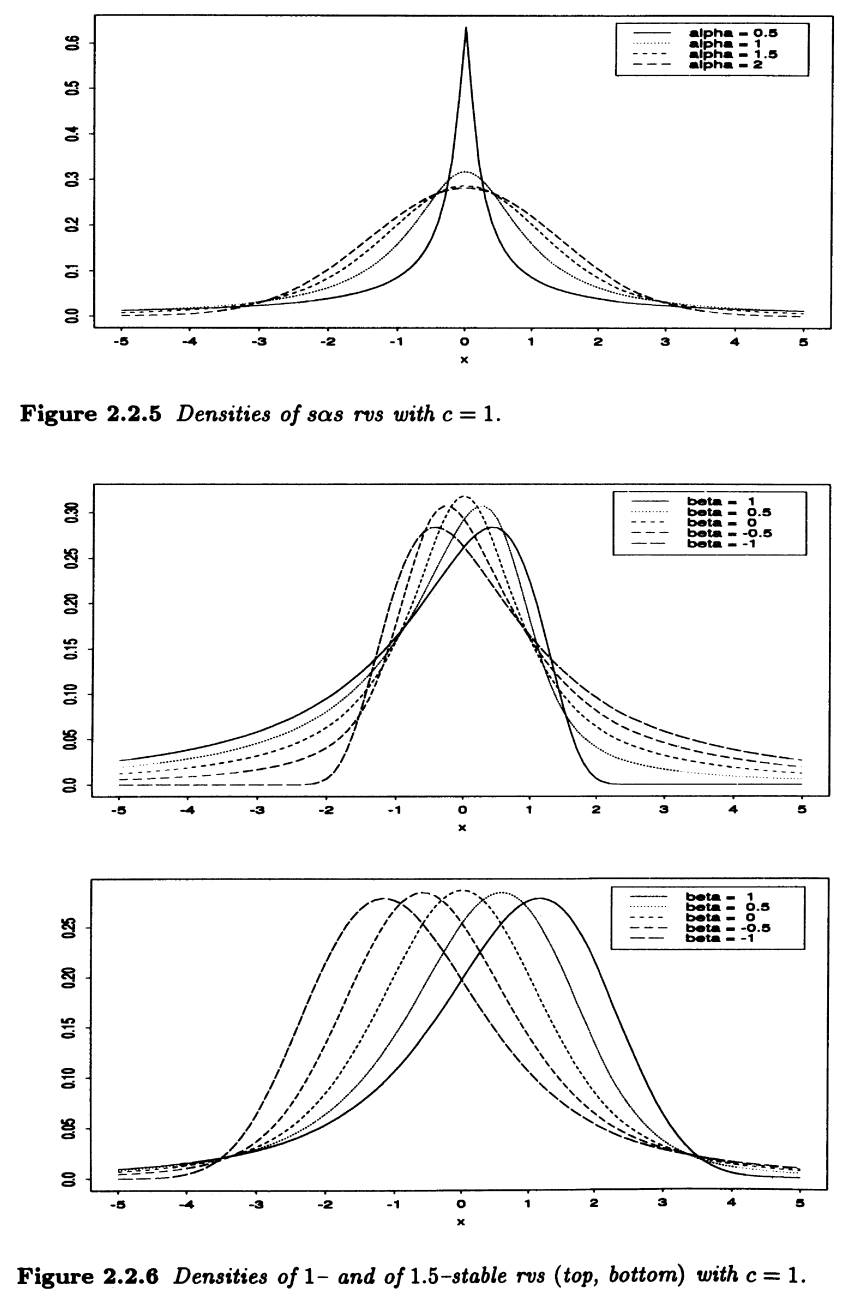
\includegraphics[height=0.68\textheight]{figures/e1-stable-parameters.png}
  \caption{稳定分布参数 $\alpha$ 与 $\beta$ 对分布形状的影响。图片来自 \cite{embrechts1997}, p.~73}
  \label{fig:e1:stable-parameters}
\end{figure}

稳定分布有非常多的应用。在金融数据、信号处理等各种领域的研究中 ，人们经常发现某些数据有 `` 高峰厚尾 '' 现象 ：数据不仅峰值高于正态分布，而且极端数据出现的频率也较大。此时用正态分布进行拟合显然是不当的，使用非正态的稳定分布来进行拟合，往往会更优。

\begin{example}[稳定分布的三个常见特例]

\begin{itemize}
\tightlist
\item
  取 $\alpha=2$ ，我们便得到了正态分布的特征函数 $e^{-ct^2}$ 。因此正态分布是一个 2-稳定分布。
\item
  取 $\alpha=1,\beta=0$ ，我们便得到了 Cauchy 分布的特征函数 $e^{-c|t|}$ 。因此 Cauchy 分布是 1-稳定分布。
\item
  若取 $\alpha=\frac12,\beta=1$ ，得到的是 \href{https://en.wikipedia.org/wiki/L\%C3\%A9vy_distribution}{Lévy 分布}，这是一个定义在正半轴上的右偏重尾分布，常用于描述 Brown 运动的首中时等。
\end{itemize}

这个例子表明，稳定分布是常见的正态分布、Cauchy 分布的推广。

虽然定理~\ref{thm:ext-stable:spectral-representation} 看起来很复杂，但事实表明，特征函数是能解析地刻画稳定分布的最好方式了 :-）对稳定分布进行统计推断的研究，基本都是从特征函数出发的，例如 \cite{feuerverger1981}、\cite{chan2009} 等。由于没有密度函数显式，因此对稳定分布的研究要困难一些，但人们还是通过很多方法得到了它的一些性质，例如，它的密度函数总是连续的，并且是单峰 (unimodal) 的；它的小于 $\alpha$ 阶矩存在，大于 $\alpha$ 阶矩不存在（见后文定理~\ref{thm:ext-stable:moments}）等。Zolotarev 的特征变换法，以及由DuMouchel 提出、Nolan 进一步发展的极大似然法\cite{nolan1997}都是稳定分布常用的估计方法。

\end{example}

\section{吸引域}

接下来的问题是，给定一个 α-稳定分布 $G_\alpha$ ，在何种条件下，随机变量的和 $S_n$ 经过适当归一化和中心化后，能收敛到 $G_\alpha$ ？

\begin{definition*}[吸引域]
设 $\{X_n\}_{n=1}^\infty$ i.i.d. 同分布于 $F$，且其部分和 $S_n$ 的极限分布是 $G_\alpha$，即存在常数 $a_n\in\mathbb R$、$b_n>0$，使得 $\frac{S_n-a_n}{b_n}\overset{\rm d}\to G_\alpha$，
那么，我们称 $F$ 属于 $G_\alpha$ 的\textbf{\emph{吸引域}} (Domain of attraction)。记作 $F \in \mathrm{DA}(G_\alpha)$。 如果只关心指数 $\alpha$，就简写为 $F \in \mathrm{DA}(\alpha)$。
\end{definition*}

下面的定理给出了完整的刻画，

\begin{definition*}[缓变函数]
$(0,\infty)$ 上（可测）的函数 $L(x)$ 若满足 $\lim_{x\to\infty}\frac{L(tx)}{L(x)}=1$，则称其为\textbf{\emph{缓变函数}} (slowly varying)。
\end{definition*}

缓变函数常见的例子是常函数和 $\ln x$ 、 $\ln\ln x$ 。

% \href{https://zhuanlan.zhihu.com/p/2024084738168603041}{【数学分析】缓慢变化函数与三个定理（一致收敛、karamata和potter上界）}

\begin{theorem}[吸引域的刻画]
\label{thm:ext-stable:domain-characterization}

\begin{itemize}
\tightlist
\item
  $\alpha = 2$ 的情形：$F \in \mathrm{DA}(2)$ 当且仅当 $\int_{|y| \le x} y^2 {\rm d}F(y)$是缓变的。
\item
  $\alpha < 2$ 的情形：$F \in \mathrm{DA}(\alpha)$（$\alpha < 2$）当且仅当存在缓变函数 $L(x)$ 以及非负常数 $c_1, c_2$（且 $c_1 + c_2 > 0$），使得\[ F(-x) = \frac{c_1 + o(1)}{x^\alpha} L(x), \quad 1 - F(x) = \frac{c_2 + o(1)}{x^\alpha} L(x), \quad x \to \infty \]
\end{itemize}

\end{theorem}

（证明见 \cite{gnedenko1954} 的第 7 章 §35，或者 \cite{ibragimov1971} 的 Theorem 2.6.1、Theorem 2.6.2。）


我们先来看第一条。若 $F$ 的二阶矩存在，那么 $L(x):=\int_{|y| \le x} y^2 {\rm d}F(y)$ 显然是一个缓变函数，因为无论是 $L(x)$ 还是 $L(tx)$ 在 $x\to\infty$ 时的极限都是 $\mathbb E[X^2],\,X\sim F$ 。所以定理~\ref{thm:ext-stable:domain-characterization} 推广了 Lindeberg--Lévy 中心极限定理。

但正态吸引域不仅限于有限二阶矩的情形。由于这两个条件是完全等价的：

\begin{itemize}
\tightlist
\item
  $\int_{|y| \le x} y^2 {\rm d}F(y)$ 是缓变函数；
\item
  $\lim\limits_{x\to\infty}\frac{x^2\int_{|y|>x}dF(y)}{L(x)} = 0$ ，即 $x^2\,P(|X|>x) = o\left(\int_{|y| \le x} y^2 {\rm d}F(y) \right)$ 。
\end{itemize}

所以定理第一条还有另一种叙述： $F$ 属于正态分布的吸引域，当且仅当

\begin{equation}
\label{eq:ext-stable:tag-1}
\frac{x^2\int_{|y|>x}\mathrm{d}F(y)}{\int_{|y|<x}y^2\mathrm{d}F(y)}\to 0\quad \text{ 当 }x\to\infty
\end{equation}

这实际上表明：就算二阶矩无穷大，尾部的质量要比``积分里的主项''小一个量级，可见正态分布的吸引域是非常广的。

再来看定理~\ref{thm:ext-stable:domain-characterization} 第二条，它表明 $\frac{F(-x)}{1-F(x)}\to \frac{c_1}{c_2}$，并且分布的左右尾部必须像 $x^{-\alpha}L(x)$ 那样衰减，换言之，$\frac{P(|X|>x)}{P(|X|>tx)}\sim t^\alpha$。相比于式~\eqref{eq:ext-stable:tag-1}，$\alpha<2$ 也有一种类似的形式：$F\in\mathrm{DA}(\alpha)$ 蕴含着存在缓变函数 $L(x)$ 使得，

\begin{equation}
\label{eq:ext-stable:tag-2}
P(|X|>x)=x^{-\alpha}L(x)
\end{equation}

且

\begin{equation}
\label{eq:ext-stable:tag-3}
\frac{x^2 P(|X| > x)}{\int_{|y|\le x} y^2 {\rm d}F(y)} \longrightarrow \frac{2 - \alpha}{\alpha}, \quad x \to \infty
\end{equation}

由式~\eqref{eq:ext-stable:tag-2} 可以看出，缓变函数 $L(x)$ 扮演着``尾部噪音''的角色；由式~\eqref{eq:ext-stable:tag-3} 可以看出，$\alpha<2$ 的 $\alpha$-稳定分布二阶矩必然为无穷（因为 $x^{2-\alpha}L(x)\to\infty$）。

进一步，我们可以得到矩的存在性结果：

\begin{theorem}[吸引域分布的矩]
\label{thm:ext-stable:moments}

若 $X\sim F \in \mathrm{DA}(\alpha)$，则：

\begin{itemize}
\tightlist
\item
  对 $0<\delta < \alpha$，$\mathbb E\big[|X|^\delta\big] < \infty$；
\item
  对 $\delta > \alpha$ 且 $\alpha < 2$，$\mathbb E\big[|X|^\delta\big] = \infty$。
\end{itemize}

特别地：

\begin{itemize}
\tightlist
\item
  当 $\alpha < 2$ 时， $\mathrm{Var}[X]=\infty$ ；
\item
  当 $\alpha > 1$ 时， $\mathbb{E}[|X|]<\infty$ ；
\item
  当 $\alpha < 1$ 时， $\mathbb{E}[|X|]=\infty$ 。
\end{itemize}

\end{theorem}

\begin{remark}

\begin{itemize}
\tightlist
\item
  定理~\ref{thm:ext-stable:moments} 第一条来自 B. V. Gnedenko，见\cite{gnedenko1954}的§35 Theorem 3 或者\cite{ibragimov1971}的 Theorem 2.6.4；第二条由式~\eqref{eq:ext-stable:tag-2} 可以直接看出。
\item
  若 $X\sim F\in\mathrm{DA}(\alpha)$ ，是可能存在 $\mathbb{E}[|X|^\alpha]<\infty$ 的。但是，若 $F$ 本身就是 $\alpha$ -稳定分布， $\alpha<2$ ，那么一定有 $\mathbb{E}[|X|^\alpha]=\infty$ 。
\end{itemize}
\end{remark}

\begin{example}[自由度为 2 的 $t$ 分布]
我们举一个简单的例子，自由度为 2 的 $t$ 分布 $t_2$ ，它的密度函数为 $f(x)=\frac1{(2+x^2)^{3/2}}$ ，容易验证其方差是不存在的：对 $X\sim t_2$ ，
\[\mathbb{E}[X^2]=\int_{\mathbb R}x^2\frac1{(2+x^2)^{3/2}}\mathrm{d}x=\infty\]
因此这个分布不满足传统 CLT 的条件。但是，我们能验证它位于正态分布的吸引域中，计算其尾部概率 \[ P(|X| > x) = 2 \int_x^\infty \frac{1}{(2+y^2)^{3/2}} \mathrm{d}y = 1 - \frac{x}{\sqrt{2+x^2}}=\frac1{x^2}+o\left(\frac1 {x^4}\right),\quad \text{ 当 }x\to\infty \]另一方面，根据 L'Hôpital 法则，
\[\lim_{n\to\infty}\frac{\int_0^x y^2f(y)\mathrm{d}y}{\ln x}=\lim_{n\to\infty}\frac{x^2f(x)}{1/x}=\lim_{n\to\infty}\frac{x^3}{(1+x^2)^{3/2}}=1\]
所以

\begin{equation}
\label{eq:ext-stable:tag-4}
\int_{|y|\le x}y^2f(y)\mathrm{d}y\sim 2\ln x
\end{equation}

由此可知，
\[
\frac{x^2P(|X|>x)}{\int_{|y|\le x}y^2f(y)\mathrm{d}y}\sim \frac{1}{2\ln x}\to 0.
\]
式~\eqref{eq:ext-stable:tag-1} 的条件满足！所以确实 $t_2\in\mathrm{DA}(2)$ 。可以证明，如果我们选择 $a_n=0$ 、 $b_n=\sqrt{n\ln n}$ ，那么
\[
\frac{S_n}{\sqrt{n\ln n}}\overset{\rm d}\to \mathcal N(0,1).
\]

这是一个``方差无限但仍然可以收敛到正态分布''的例子。


\end{example}

\section{归一化和中心化常数应该怎么选？}

\subsection{归一化常数}

首先，如果 $X$ 的分布是对称 $\alpha$ -稳定的，那么其特征函数为 $e^{-c|t|^\alpha}$ ，我们注意到
\[\begin{aligned} \phi_{n^{-1/\alpha}S_n}(t)&=\mathbb{E}[\exp \{itn^{-1/\alpha }S_n\}]\\ &=(\phi_X(n^{-1/\alpha }t))^n \\ &=\left(\exp\left\{-c|n^{-1/\alpha} t|^\alpha\right\}\right)^n\\ &=\exp\{-c|t|^\alpha\}\\ &=\phi_{X}(t) \end{aligned}\]
于是 $n^{-1/\alpha}S_n\overset{\rm d}=X$ 。所以直觉上 $b_n = n^{1/\alpha}$ 是合适的归一化项。

对于一般的吸引域中的 $X$，特征函数在 $0$ 附近的行为是 $\exp\{ -|t|^\alpha L_1(1/t) \}$，其中 $L_1$ 缓变（\cite{ibragimov1971} 的 Theorem 2.6.5），于是归一化项需要包含一个缓变修正：
\[b_n = n^{1/\alpha} L_2(n)\]
直观上，对于一个属于 $\mathrm{DA}(\alpha)$ 但不一定是稳定分布的 $X$，它的尾部可能不是纯幂律，而是 $P(|X|>x) \sim x^{-\alpha} L(x)$ （式~\eqref{eq:ext-stable:tag-3} ）。这时，若仍取 $b_n = n^{1/\alpha}$就不太够了，因为 $L$ 可能会把依分布收敛破坏掉；必须加上一个修正，从而将 $L(x)$ 的影响吸收掉。

为了更精确地构造 $b_n$，我们定义两个辅助函数：
\[K(x) := x^{-2} \int_{|y|\le x} y^2 {\rm d}F(y), \quad Q(x) := P(|X| > x) + K(x), \quad x > 0\]
那么，可以取 $b_n$ 为方程 $Q(b_n) = n^{-1}$ 的唯一解，或者渐近意义上是方程解。特别地，

\begin{itemize}
\tightlist
\item
  如果 $\sigma^2 = \mathrm{Var}[X] < \infty$ 且 $\mathbb E[X] = 0$，那么 $P(|X|>x)=o(x^{-2})$ 、 $K(x)=x^{-2}\mathbb{E}[X^2](1+o(1))$ 。此时若 $n^{-1}\sim Q(b_n)\sim b_n^{-1}\sigma^2$ ，我们可以直接选取 $b_n =n^{1/2} \sigma$。
\item
  如果 $\alpha < 2$，我们可以取 $b_n = \inf\{ y : P(|X| > y) < n^{-1} \}$，此时 $P(|X| > b_n) \sim n^{-1}$，并且 式~\eqref{eq:ext-stable:tag-2}告诉我们 $b_n = n^{1/\alpha} L_3(n)$，$L_3$ 缓变。 那么，根据式~\eqref{eq:ext-stable:tag-3} ， $K(x) \sim \frac{\alpha}{2-\alpha}P(|X|>x)$ ，于是\[ Q(x) = P(|X|>x)+ K(x) \sim \left(1 + \frac{\alpha}{2-\alpha}\right) P(|X|>x) = \frac{2}{2-\alpha} P(|X|>x) \] 即 $Q(x)$ 与 $P(|X|>x)$ 相差一个常数倍， $P(|X| > b_n) \sim n^{-1}$ 已经足够。
\end{itemize}

为什么要让 $Q(b_n)\sim n^{-1}$ 呢？直观上，对于重尾分布，和 $S_n$ 的渐近行为由两部分共同决定：

\begin{itemize}
\tightlist
\item
  ``大量微小震荡''（$|X_i| \le b_n$）：这部分累积的方差贡献由 $K(x)$ 描述。
\item
  ``单次巨大跳跃''（$|X_i| > b_n$）：这部分由 $P(|X|>x)$ 描述。
\end{itemize}

如果我们希望标准化后的和 $\frac{S_n - a_n}{b_n}$ 收敛到某个非退化极限分布，就需要让上述两种贡献加起来后的总波动能在尺度 $b_n$ 下得以被控制，这就是让 $nP(|X|>b_n)+nK(b_n)=nQ(b_n)=1$ 的含义。

% （当然这个只是直觉上的解释，理论上应该也是可以进行推导的。）

读者可以看图~\ref{fig:e1:partial-sum-paths}，对于标准正态分布， $S_n$ 总体上是比较连续的；而对于诸如标准 Cauchy 这样的重尾分布，由于极端值更可能出现， $S_n$ 会产生比较大的跳跃：

\begin{figure}[htbp]
  \centering
  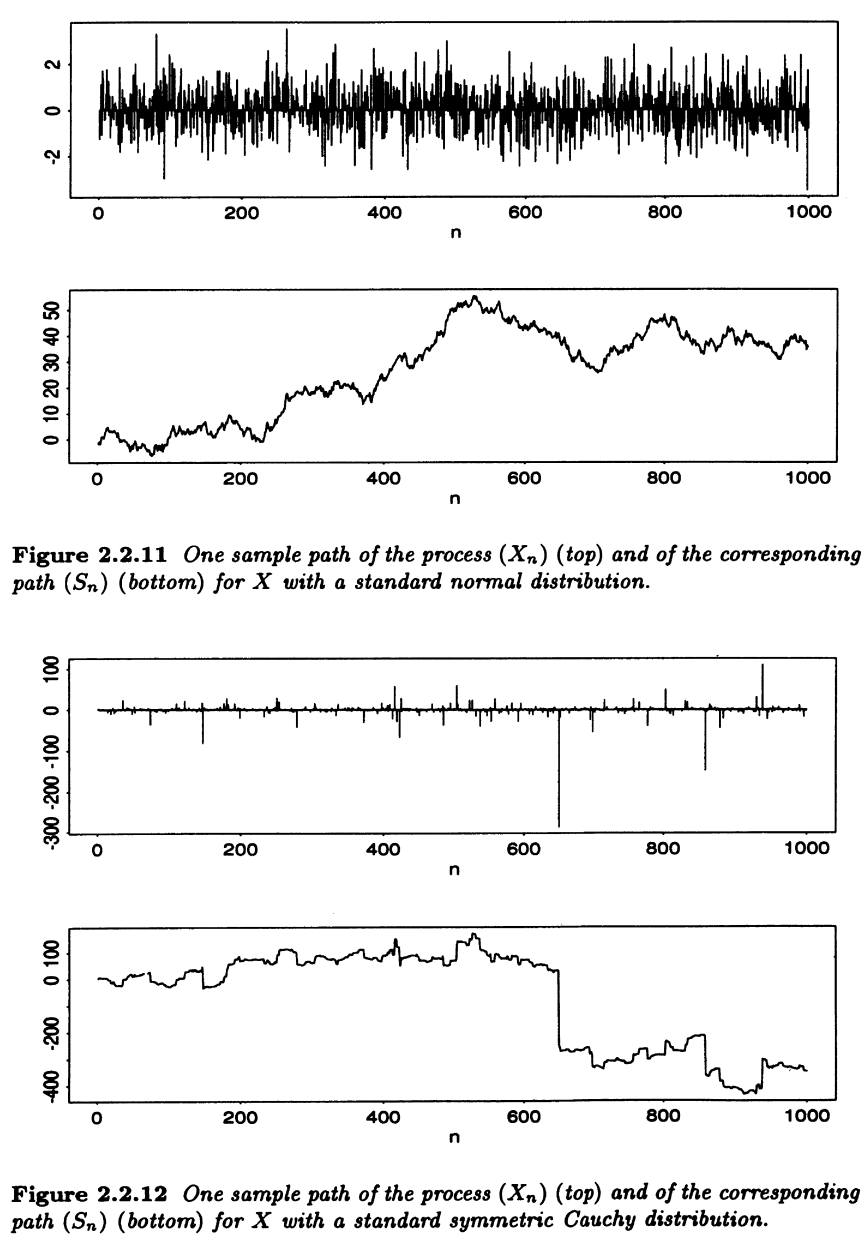
\includegraphics[height=0.68\textheight]{figures/e1-partial-sum-paths.png}
  \caption{正态分布与重尾分布的部分和路径。图片来自 \cite{embrechts1997}, p.~77}
  \label{fig:e1:partial-sum-paths}
\end{figure}

这背后隐含着重尾分布的一个核心直觉：``单次大跳跃原理 (Single Big Jump Principle)''。在经典的正态中心极限定理中，和 $S_n$ 的波动是由大量微小的独立震荡累积而成的；但在 Cauchy 等重尾分布中，和 $S_n$ 的极端波动往往是由某一个或极少数几个极端的观测值主导的。

\begin{example}[$t_2$ 分布的归一化常数]
继续前文的 $t_2$ 分布。式~\eqref{eq:ext-stable:tag-1} 告诉我们 $P(|X|>x)/K(x)\to 0$ ，因此 $Q(x)=P(|X|>x)+K(x)\sim K(x)$ 。式~\eqref{eq:ext-stable:tag-4} 告诉我们 $K(x)\sim \frac{2\ln x}{x^2}$ ，于是方程 $Q(b_n)\sim K(b_n)\sim n^{-1}$ 化作 $b_n^2\sim 2n\ln b_n$ ，容易看出 $b_n=\sqrt{n\ln n}$ 是满足的。

\end{example}


\subsection{中心化常数}

中心化常数 $a_n$ 的选择是下述截断均值： $a_n=n\int_{|y|\le b_n}y\mathrm{d}F(y)$或者渐近意义上使得上式成立；其中 $b_n$ 由上节的方法确定。之所以要用截断均值，是因为总体均值 $\mathbb{E}[X]$ 在 $\alpha\le 1$ 时是不存在的，不能简单地用 $n\mathbb {E}[X]$ 来中心化，我们只能退而求其次，对那些``不太大''（ $|y|\le b_n$ ）的项进行中心化对齐。

\begin{itemize}
\tightlist
\item
  不过，一种简单的情形是，如果分布是对称的，例如关于 0 对称，我们可以直接取 $a_n=0$ 。
\item
  对 $1<\alpha\le 2$ 的情况，由于均值 $\mu$ 存在且 $\int_{|y|\le b_n}y\mathrm{d}F(y)\to \mu$ ，我们取 $a_n=n\mu$ 即可。
\end{itemize}

\section{广义中心极限定理}

把上面所有的准备工作合并起来，我们就得到了最完整的结论：

\begin{theorem}[广义中心极限定理]
\label{thm:ext-stable:gclt}

设 $F \in \mathrm{DA}(\alpha)$，$\alpha \in (0,2]$。

\begin{itemize}
\tightlist
\item
  二阶矩有限情形（此时必有 $\alpha=2$ ）：如果 $\mathbb{E}[X^2]<\infty$ ，则
  \[
  \frac{S_n - n\mu }{\sigma n^{1/2}} \overset{\rm d}\to \mathcal N(0,1).
  \]
\item
  如果 $\mathbb E[X^2] = \infty$ 且 $\alpha = 2$，或者 $\alpha < 2$，那么存在缓变函数 $L_4(n)$ 和 (上节中定义的) 序列 $a_n$，使得
  \[
  \frac{S_n-a_n}{n^{1/\alpha}L_4(n)}\overset{\rm d}\to G_\alpha,
  \]
  其中 $G_\alpha$ 是一个 $\alpha$-稳定分布。
\end{itemize}

\end{theorem}

在某些特殊情况下，归一化常数 $b_n=n^{1/\alpha}L_4(n)$ 中的缓变函数 $L_4(n)$ 可以吸收为一个常数，即 $b_n = c n^{1/\alpha}$。这时我们称分布属于 \textbf{\emph{正规吸引域}} (domain of normal attraction)。

\begin{definition*}[正规吸引域]
如果分布 $F\in\mathrm{DA}(G_\alpha)$ 且可以选取 $b_n=cn^{1/\alpha}$（$c>0$ 为常数）使得 $\frac{S_n-a_n}{b_n}\overset{\rm d}\to G_\alpha$ 成立，则称 $F$ 属于 $G_\alpha$ 的\textbf{\emph{正规吸引域}}，记作 $F\in\mathrm{DNA}(G_\alpha)$ 或 $F\in\mathrm{DNA}(\alpha)$。
\end{definition*}

根据我们前文对归一化常数选取的分析，以及定理~\ref{thm:ext-stable:domain-characterization}，推知

\begin{theorem}[正规吸引域的刻画]
\label{thm:ext-stable:normal-domain-characterization}

\begin{itemize}
\tightlist
\item
  当 $\alpha = 2$ 时：$F \in \mathrm{DNA}(2)$ 当且仅当 $\mathbb E[X^2] < \infty$。
\item
  当 $\alpha < 2$ 时：$F \in \mathrm{DNA}(\alpha)$ 当且仅当存在非负常数 $c_1, c_2$（$c_1 + c_2 > 0$）使得
  \[
  F(-x) \sim c_1 x^{-\alpha}, \quad 1 - F(x) \sim c_2 x^{-\alpha}, \quad x \to \infty.
  \]
\end{itemize}

\end{theorem}

也就是说，正规吸引域中，分布的尾部是纯幂律的，不需要缓变函数进行修正。特别地，所有 $\alpha$ -稳定分布都在它自己的正规吸引域中。
 
